\section{\PwTerTITLE: automatic litmus test evaluator}
\label{sec:tool}

\PwTer{} automatically and exhaustively calculates the allowed outcomes of litmus tests for the \PwT, \PwTpo, and \PwTc{} models. It is built in OCaml, and uses Z3~\cite{Z3Solver} to judge the truth of predicates constructed by the models. \PwTer{} obviates the need for error-prone hand evaluation.

\PwTer{} allows several modes of evaluation: it can evaluate the rules of Fig.~\ref{fig:seq}, implementing \PwT; it can generate program order according to Section~\ref{sec:c11}, implementing \PwTpo; and similar to \MRD~\cite{DBLP:conf/esop/PaviottiCPWOB20}, it can construct C11-style pre-executions and filter them according to the rules of C11.
Our choice of C11 rules is careful: we take the rules of RC11~\cite{DBLP:conf/pldi/LahavVKHD17}, but we replace the overly strong No-Thin-Air restriction $\text{acyclic}(\rrf\cup\rpox)$ with $\text{acyclic}(\rrf\cup\lt)$. 
This is a more precise categorisation of thin-air behavior, and it allows aggressive compiler optimizations which would be erroneously forbidden by RC11's original No-Thin-Air axiom.
We show \PwTer{} in action in Fig.~\ref{fig:tool}.
Finally, \PwTer{} also allows us to toggle the complete check of~\ref{def:pomset}, providing an interface for understanding how fragments of code might compose by exposing preconditions and termination conditions which are not yet tautologies.

%% TODO: introduce some nice dogma about the value of a tool and what it's taught us.
%% The real friends are the tools we built along the way.

%% Notes for Simon and Mark:
% Intro
%  - Add contribution relating to tool

% Related work
%  - Mention tool for MRD & Event Structures, mention absence of tool for Promising

% This section
%  - tool for {PwT, PwT-PO, PwT-RC11}
%  - Validation of some tests? Which tests to include?

% C11 Section
%  - Discussion: C11 standard really needs a dep relation. MRD provides this, PwT provides this, Promising does not.
%  - There's an open question about how coherence should affect dep.
%    if(q) { x := 1; x := 2 } else { x := 2; x := 1 }
%  - What should the deps be?

% Conclusion
%  - Having a tool should be some kind of feel-good factor.

%% [Simon] I am not a fan of how this looks on the page.
\begin{figure}[t]
\begin{center}
  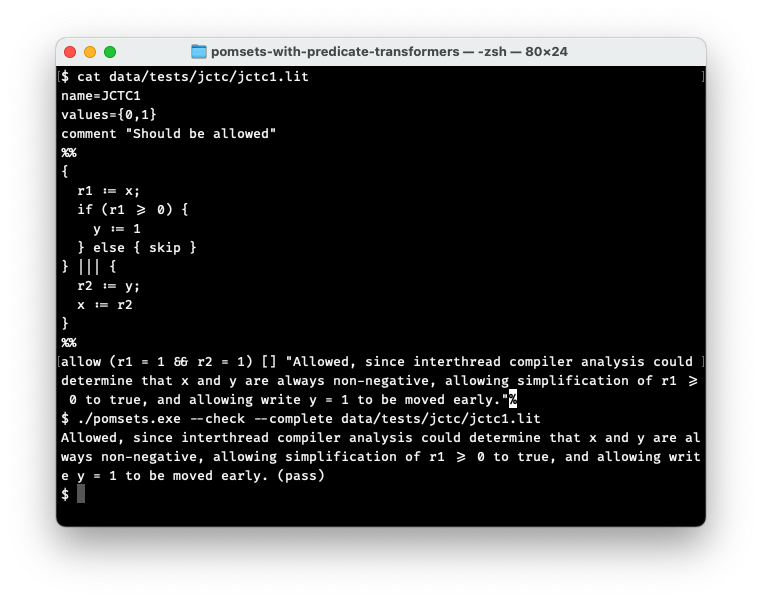
\includegraphics[width=0.75\textwidth]{tool.png}
  \Description{Image shows tool running on a Mac. Java Causality Test Case 1 is printed, followed by an invocation of the tool as {\tt ./pomsets.exe --check --complete data/tests/jctc/jctc1.lit}, which shows that the tool passes the assertion listed in the test.}
  \caption{\label{fig:tool} Example output of \PwTer, validating TC1~\cite{PughWebsite}.}
\end{center}
\end{figure}
